\documentclass[ngerman,aspectratio=169]{beamer}
\usepackage[utf8]{luainputenc}
\usepackage[TS1,T1]{fontenc}
\usepackage{babel}
\usetheme[pagenum,navbar,ddc]{tud}
\usepackage{xcolor}
\usepackage{listings}
\usepackage{tikz}
\usepackage{multicol}
\usepackage[labelformat=empty,font=scriptsize]{caption}

\newcommand{\theory}[1]{\text{Th(} #1 \text{)}}
\newcommand{\lang}[1]{\text{L(}#1{)}}

\title{TUN/TAP-Geräte\protect\\\mdseries Übersicht, Funktionsweise und Implementierung im Linux-Kernel\strut}
\subtitle{Proseminar Rechnernetze}
\author{Lucas Waclawczyk}

\newcommand*\inmm[1]{\pgfmathsetmacro\inmmwert{#1 / 1mm}\inmmwert}
\makeatletter
\newcommand*\inpt[1]{\setlength\@tempdima{#1}\the\@tempdima}
\makeatother

\AtBeginSection[]{\partpage{\usebeamertemplate***{part page}}}
\begin{document}
	\mode<presentation>{\setbeamertemplate{tud background}[image/shaded]{Seminarraum.jpg}{0.7}}
	\maketitle
	
	\mode<presentation>{\setbeamertemplate{page number in footline}[frame][text and total]}
	\frame{\frametitle{Inhalt}\tableofcontents}
	
	\section{Übersicht}
	\subsection{Rückblick Network Interfaces}
	\begin{frame}{Rückblick Network Interfaces}
		\begin{multicols}{2}
			\begin{itemize}
				\setlength{\itemsep}{1em}
				\item Interface = Schnittstelle
				\item muss nicht physisch sein\\(Virtual Network Interface)
			\end{itemize}
			\only<1>{
				\begin{figure}
					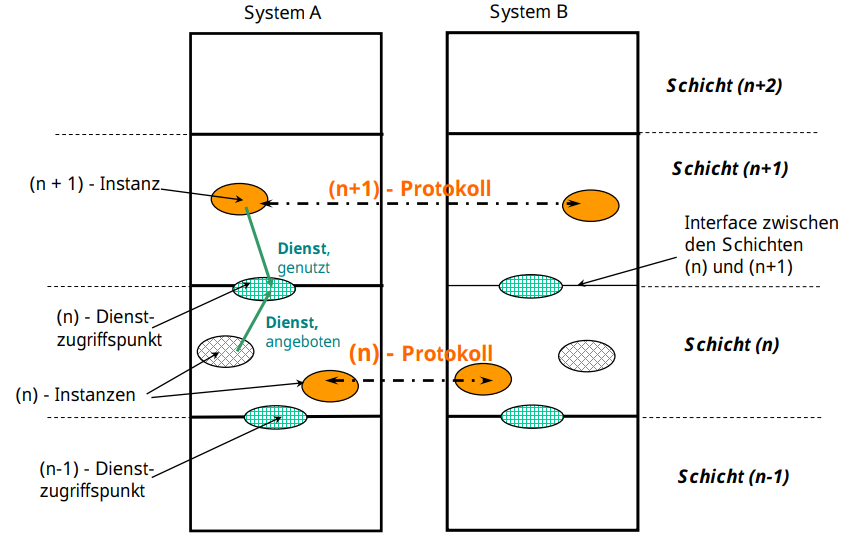
\includegraphics[width=\linewidth]{network_interface}
					\caption{aus \hyperlink{src:rene}{[1]}}
				\end{figure}
			}
			\only<2>{
				\begin{figure}
					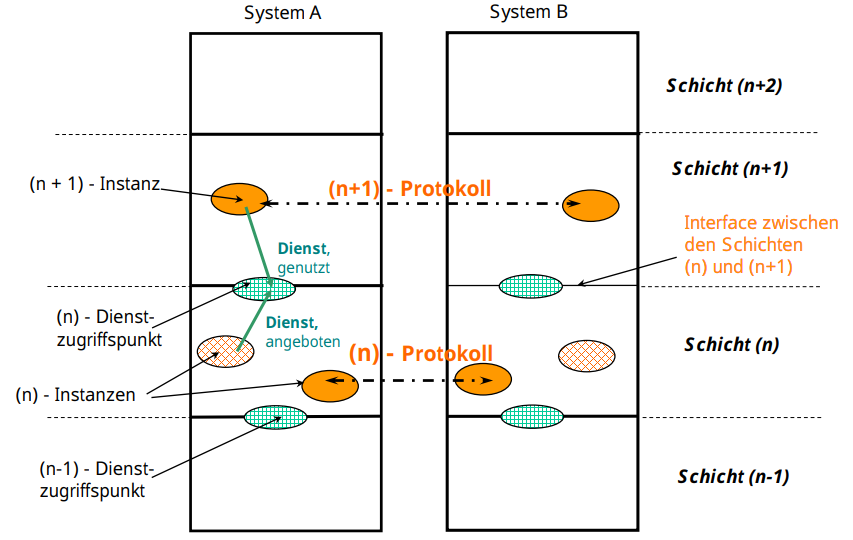
\includegraphics[width=\linewidth]{network_interface_colored}
					\caption{aus \hyperlink{src:rene}{[1]}}
				\end{figure}
			}
		\end{multicols}
	\end{frame}

	\subsection{Gemeinsamkeiten von TUN und TAP}
	\begin{frame}{Generelles zu TUN und TAP}
		\begin{itemize}
			\item Virtual Network Interfaces
			\begin{itemize}
				\item IP-Adresse
				\item Traffic analysieren
				\item Firewall-Regeln
			\end{itemize}
			\item \textit{OS $ \leftrightarrow $ Anwendung} statt \textit{physische Verbindung $ \leftrightarrow $ Hardware}
			\item u. A. Linux, Windows 2000 - 10, Mac OS X (nur TUN eingebaut)
			\item hier für Linux
		\end{itemize}
	\end{frame}

	\subsection{Unterschiede zwischen TUN und TAP}
	\begin{frame}{Unterschiede zwischen TUN und TAP}
		\renewcommand{\arraystretch}{1.5}
		\begin{tabular}{p{.5\linewidth}|p{.5\linewidth}}
			\textbf{TUN} & \textbf{TAP} \\\hline
			"Netzwerk-Tunnel" & "Terminal Access Point"\\\hline
			IP-Pakte & Ethernet-Frames\\\hline
			Ende zu Ende & Punkt zu Punkt
		\end{tabular}
	\end{frame}

	\section{Funktionsweise}
	\subsection{Set Up}
	\begin{frame}{Set Up}
		\begin{itemize}
			\item \texttt{/dev/net/tun} (Clone Device) öffnen (r, w)
			\item \texttt{struct flag\_struct} mit Name, \texttt{TUN\_IFF} oder \texttt{TAP\_IFF}
			\item Systemaufruf: \texttt{ioctl(fd, TUNSETIFF, flag\_struct)}
			\item evtl. persistent einrichten
		\end{itemize}
	\end{frame}

	\subsection{Workflow}
	\begin{frame}{Workflow}
		\begin{itemize}
			\item Daten wie gewöhnlich an Interface gesendet
			\item Lesen durch \texttt{fd}
			
			\item Vorteile
			\begin{itemize}
				\item gut konfigurierbar
				\item verhält sich wie echter Netzwerkadapter
			\end{itemize}
			\item Nachteile
			\begin{itemize}
				\item ineffizient
				\item langsamer als Heimnetz (schwächstes Glied)
			\end{itemize}
		\end{itemize}
	\end{frame}

	\subsection{Tear Down}
	\begin{frame}{Tear Down}
		\begin{itemize}
			\item \emph{transientes} Gerät verschwindet bei Beenden der angebundenen Anwendung
			\item \emph{persistentes} Gerät muss aktiv abgebaut werden
		\end{itemize}
	\end{frame}

	\section{Implementierung}
	\subsection{Wo findet man das?}
	\begin{frame}{Wo findet man das?}
		\begin{itemize}
			\item Kernel-Code: \url{https://github.com/torvalds/linux.git}
			\item TUN: \texttt{/linux/drivers/net/tun.c}
			\item Clone Device: \texttt{/dev/net/tun}
		\end{itemize}
	\end{frame}
	
	\subsection{Code}
	\begin{frame}{Code}
		etwa drei Folien
	\end{frame}

	\section{Quellen}
	\begin{frame}{Quellen}
		\begin{enumerate}
			\item[{[1]}] Skript und Übungsaufgaben der Vorlesung Rechnernetze, TU Dresden 2019 (präzise genug?) \label{src:rene}
			\item[{[2]}] \url{https://backreference.org/2010/03/26/tuntap-interface-tutorial/}
			\item[{[3]}] \url{https://www.elektronik-kompendium.de/sites/net/0811011.htm}
			\item[{[4]}] \url{https://en.wikipedia.org/wiki/TUN/TAP}
			\item[{[5]}] \url{https://www.thomas-krenn.com/de/wiki/OpenVPN_Grundlagen}
		\end{enumerate}
\end{frame}
\end{document}
